\section{Implementation and Prototypes}
This research was originally born from the willingness to explore the possibility of exploiting the technology of flexible coil inductors by using one produced by the research group \textbf{Helmholtz-Zentrum Dresden-Rossendorf} (HZDR) in Dresden, Germany \cite{HZDR}.
After testing this coil, we realized its \textbf{limitations} and decided to explore other alternatives, such as flexible PCB coils.
Flexible PCB coils are much sturdier than the HZDR coil, easily designable and manufacturable, and have a much higher power rating.
The low power rating meant that the HZDR coil was not able to generate a magnetic field strong enough for our application.

\subsection{Rigid Prototype}
The first prototype was designed to test the capabilities of the Dresden coils.
In the previous research done by the HZDR team, they tested the coil using a simple piece of \textbf{flexible magnetic tape as a membrane}.
This membrane is shaped like a "fish" so the tail can be fixed on a plane and the head can be \textbf{free to bend} up and down.
\begin{figure}[H]
    \centering
    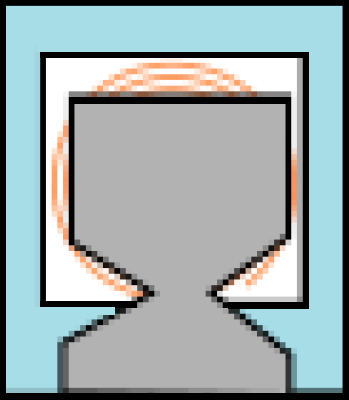
\includegraphics[width = 0.2\linewidth]{Figures/Dresden_test.png}
    \caption{Dresden coil HZDR test setup}
    \label{fig: Dresden_test}
\end{figure}
The pulp needed to be suspended at a certain distance to \textbf{avoid pressing} on the membrane, this would have caused the membrane to \textbf{stop vibrating}.

To solve this problem we developed a structure able to keep the coil and membrane at a certain distance from the pulp.
\begin{figure}[H]
    \centering
    \begin{subcaptiongroup}
      \centering
      \parbox[b]{0.2\textwidth}{
        \centering
        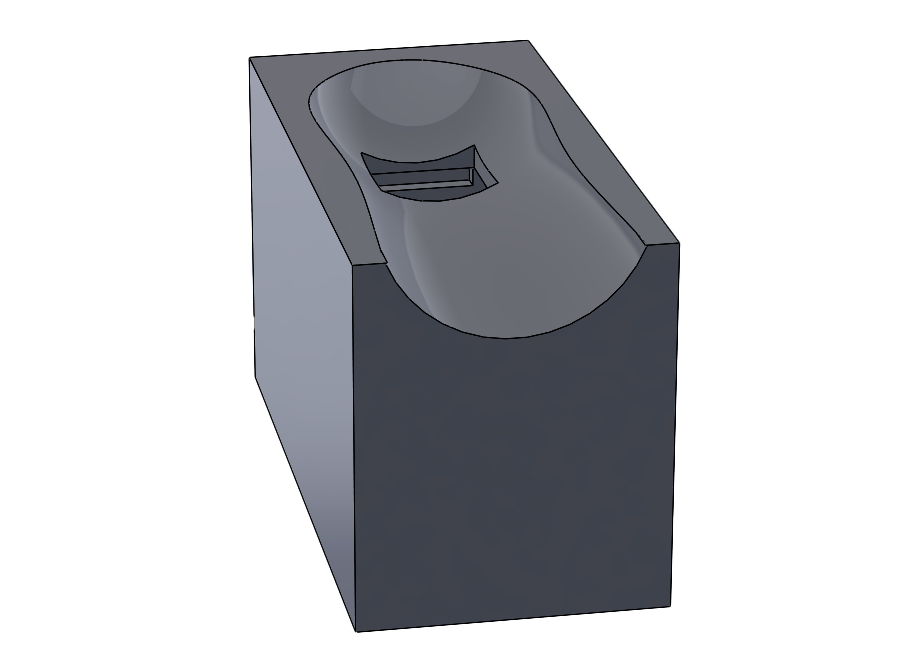
\includegraphics[width = 0.9\linewidth]{Figures/finger_holder.png}
        \caption{Finger resting surface}
      }
      \parbox[b]{0.2\textwidth}{
        \centering
        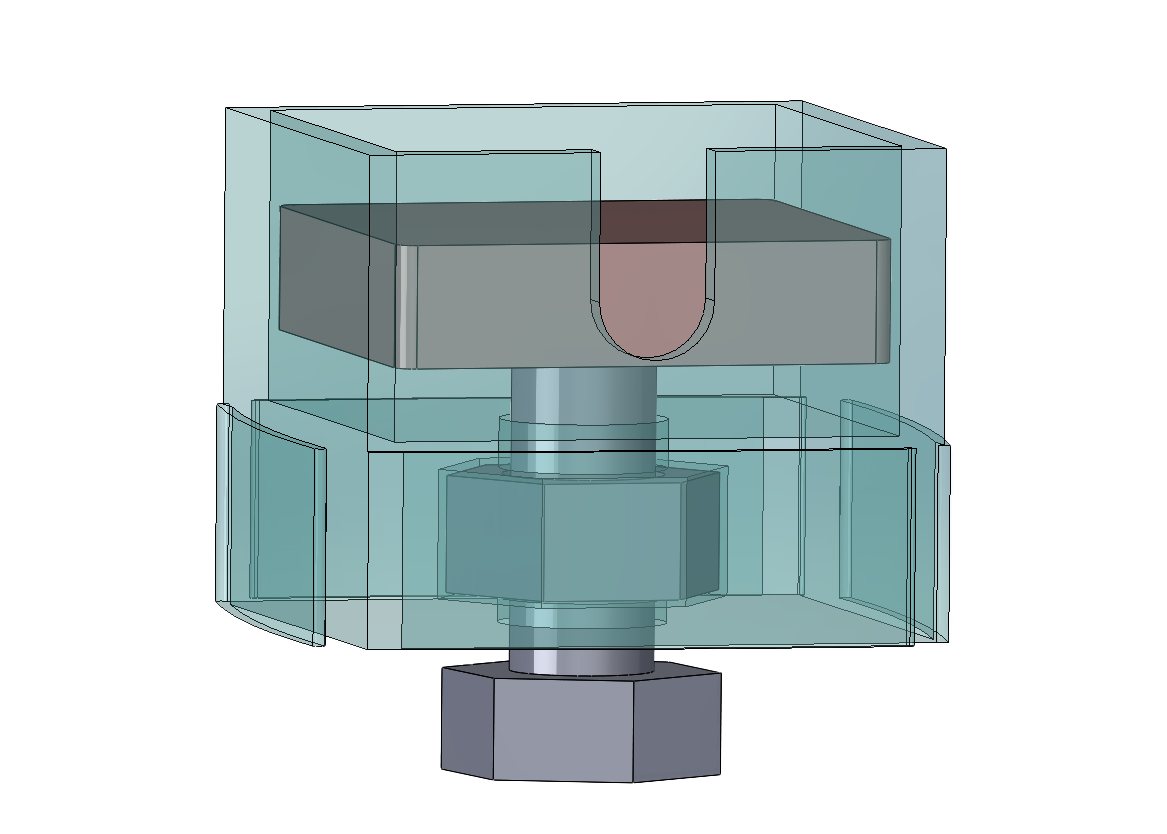
\includegraphics[width = 0.9\linewidth]{Figures/adj_platform.png}
        \caption{Finger platform}
      }
    \end{subcaptiongroup}
    \caption{Components of the first prototype}
\end{figure}
The coil and the membrane are placed on top of the height-adjustable platform, then the finger would lay on the hole of the resting surface.

\subsection{Wearable Rigid Prototype}
The following prototype was based on the flexible PCB coil. A structure was designed to keep the coil in place and allow it to be worn on the finger through the use of silicon sleeves.
This sleeve was designed to be adaptable to different finger sizes and to integrate a cylindrical magnet on the pulp.
\begin{figure}[H]
    \centering
    \begin{subcaptiongroup}
        \centering
        \parbox[b]{0.2\textwidth}{
            \centering
            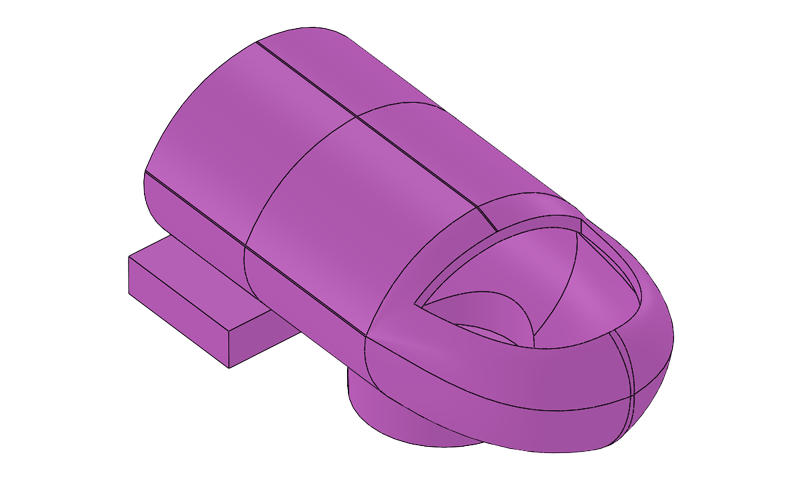
\includegraphics[width=0.2\textwidth]{Figures/silicon_sleeve_front.png}
        }
        \parbox[b]{0.2\textwidth}{
            \centering
            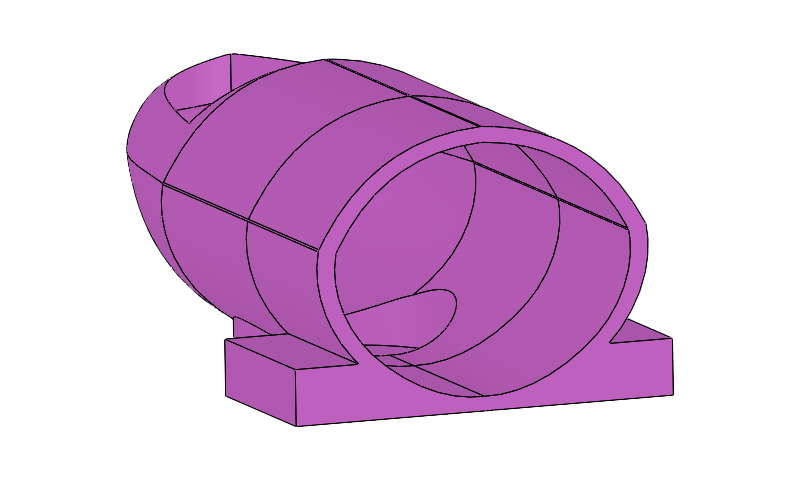
\includegraphics[width=0.2\textwidth]{Figures/silicon_sleeve_back.png}        
        }
    \end{subcaptiongroup}
    \caption{Finger silicon sleeve front and back view}
\end{figure}
The silicon sleeve could be then connected to the assembly where the coil and heatsink were placed through its lateral mounting wings.
\begin{figure}[H]
    \centering
    \begin{subcaptiongroup}
        \centering
        \parbox[b]{0.2\textwidth}{
            \centering
            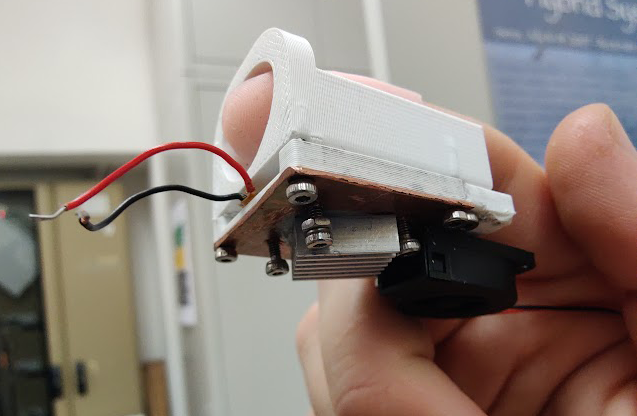
\includegraphics[width=0.2\textwidth]{Figures/rigid_prot_btm.png}
        }
        \parbox[b]{0.2\textwidth}{
            \centering
            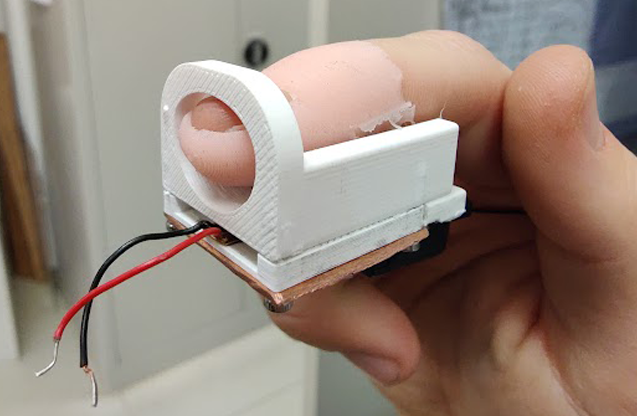
\includegraphics[width=0.2\textwidth]{Figures/rigid_prot_top.png}
        }
    \end{subcaptiongroup}
    \caption{Bottom and top view of the real prototype}
\end{figure}
This prototype is much better than the previous one, the magnet was kept at the right distance from the coil and the vibrations were much more noticeable, also being wearable made it much easier to use.
Its biggest problem was the silicon sleeve, as the silicon tends to absorb some of the vibrations and the softness of the material made the mounting mechanism a bit finicky.  
We also had to add a small blowing fan to the heatsink to keep the coil cool as it would heat a lot after a few minutes of use.

\subsection{Flexible Mat Prototypes}
The final prototype was designed to be a flexible silicon mat where all components were integrated, including the membrane.

